%%%%%%%%%%%%%%%%%%%%%%%%%%%%%%%%%%%%%%%%%%%%%%%%%%%%%%%%%%%%%%%%%%%%%%%%%%%%%%%%%%
\begin{frame}[fragile]\frametitle{}
\begin{center}
{\Large Introduction}
\end{center}
\end{frame}

% %%%%%%%%%%%%%%%%%%%%%%%%%%%%%%%%%%%%%%%%%%%%%%%%%%%%%%%%%%%%%%%%%%%%%%%%%%%%%%%%%%
% \begin{frame}[fragile]\frametitle{Objective}

% Graph query languages, while precise and powerful, can sometimes be challenging to comprehend and employ. 
% However, employing natural language to construct and query graphs presents an ideal alternative. 
% This approach is particularly suitable for Knowledge Graphs derived from textual data. 
% This presentation explores the foundation, methodologies, and illustrative instances of utilizing LLMs to enhance KGs.


% \end{frame}

% %%%%%%%%%%%%%%%%%%%%%%%%%%%%%%%%%%%%%%%%%%%%%%%%%%%%%%%%%%%
% \begin{frame}[fragile]\frametitle{Augmenting LLMs with Knowledge Graphs: Motivation}

% \begin{itemize}
% \item The Butcher-on-the-Bus: Rhetorical device highlighting human memory processes.
% \item Memory Types: Two types of memory: flexible, fuzzy, and gradually learned vs. specific, precise, and acquired in a single shot.
% \item Enhancing AI Systems: LLMs offer generalization and creativity but suffer from hallucinations, unreliability, and staleness. Databases provide accuracy and reliability but lack adaptability and intelligence.
% \item Bridging the Gap: Integrating LLMs with Knowledge Graphs (KGs) to create a Working Memory Graph (WMG) combines the strengths of both approaches.
% \item WMG Construction: LLM processes a question, returns a graph of nodes using URLs as identifiers, and links to ground truths in the KG. Conceptual understanding nodes connect LLM's vectors with KG's ontological classes.
% \item Favorable Direction: Combining LLMs' reasoning capabilities with KGs' structured ontology can lead to promising exploration.
% \end{itemize}

% Thus, combining the best of both worlds (LLMs with their reasoning capabilities along with KGs with their structured, static ontology) can yield a favorable direction to explore.

% {\tiny (Ref: Per Tony Seale, Overview of Large Language Models - Aman AI)}

% \end{frame}

%%%%%%%%%%%%%%%%%%%%%%%%%%%%%%%%%%%%%%%%%%%%%%%%%%%%%%%%%%%
\begin{frame}[fragile]\frametitle{Limitations of Large Language Models in the Enterprise Context}

\begin{itemize}
\item Hallucinations: LLMs generate plausible but inaccurate responses.
\item Misinformation: LLMs unintentionally perpetuate false information.
\item Biases: LLMs exhibit biases from training data, impacting decision-making.
\item Cut-off: LLMs lack awareness of events after their training.
\item Corpus: LLMs lack knowledge of events not in their training data.
\item Fine-tuning mitigates but doesn't eliminate hallucinations.
\item LLMs don't cite sources, lack access restrictions.
\end{itemize}	

\end{frame}

%%%%%%%%%%%%%%%%%%%%%%%%%%%%%%%%%%%%%%%%%%%%%%%%%%%%%%%%%%%
\begin{frame}[fragile]\frametitle{Solution for Limitations}

\begin{itemize}
\item Fine-tuning: Supervised training phase to optimize LLM performance.
\item Use case 1: Updating and expanding internal knowledge.
\item Use case 2: Fine-tuning for specific tasks (e.g., summarization, translation).
\end{itemize}	

\end{frame}


%%%%%%%%%%%%%%%%%%%%%%%%%%%%%%%%%%%%%%%%%%%%%%%%%%%%%%%%%%%
\begin{frame}[fragile]\frametitle{Knowledge Graphs as Support Mechanisms for LLMs}

\begin{itemize}
\item Knowledge Graphs: Structured representation using nodes and edges.
\item Interface with LLMs: Integrates Knowledge Graphs with LLMs.
\item Enables access to structured data.
\item Enhances LLM outputs.
\item Benefits of Integration: Mitigates LLM limitations.
\item Provides accurate, context-specific, unbiased information.
\end{itemize}	

\end{frame}



%%%%%%%%%%%%%%%%%%%%%%%%%%%%%%%%%%%%%%%%%%%%%%%%%%%%%%%%%%%%%%%%%%%%%%%%%%%%%%%%%%
\begin{frame}[fragile]\frametitle{}
\begin{center}
{\Large Knowledge Graph (KG)}

\end{center}
\end{frame}

%%%%%%%%%%%%%%%%%%%%%%%%%%%%%%%%%%%%%%%%%%%%%%%%%%%%%%%%%%%%%%%%%%%%%%%%%%%%%%%%%%
%%%%%%%%%%%%%%%%%%%%%%%%%%%%%%%%%%%%%%%%%%%%%%%%%%%%%%%%%%%
\begin{frame}[fragile]\frametitle{What is KG?}

\begin{itemize}
\item A knowledge graph is a graph-based database that represents knowledge in a structured and semantically rich format. 
\item This could be generated by extracting entities and relationships from structured or unstructured data, such as text from documents. 
\item A key requirement for maintaining data quality in a knowledge graph is to base it on standard ontology. 
\item Having a standardized ontology often involves the cost of incorporating this ontology in the software development cycle.
\end{itemize}

\end{frame}



%%%%%%%%%%%%%%%%%%%%%%%%%%%%%%%%%%%%%%%%%%%%%%%%%%%%%%%%%%%%%%%%%%%%%%%%%%%%%%%%%%
\begin{frame}[fragile]\frametitle{}
\begin{center}
{\Large Generative AI - Large Language Models (LLMs)}

\end{center}
\end{frame}


%%%%%%%%%%%%%%%%%%%%%%%%%%%%%%%%%%%%%%%%%%%%%%%%%%%%%%%%%%%%%%%%%%%%%%%%%%%%%%%%%%
%%%%%%%%%%%%%%%%%%%%%%%%%%%%%%%%%%%%%%%%%%%%%%%%%%%%%%%%%%%
\begin{frame}[fragile]\frametitle{What is LLM?}

\begin{itemize}
\item Large Language Models (LLMs): Machine learning algorithms for interpreting, translating, and summarizing natural language texts.
\item Size: Span hundreds of gigabytes with trillions of parameters.
\item Deep neural networks: Learn from extensive training data to generate appropriate outputs.
\item Self-attention mechanisms: Capture relationships between words, even with incorrect positioning.
\item Transformer architecture: Implements self-attention mechanisms.
\item Training data: Accumulated from multiple sources (books, internet, articles, social media, research papers).
\item Applications: Conversational AI, content creation engines, search engines, customer service agents, etc.
Enhance natural language processing tasks.
\end{itemize}

\end{frame}

%%%%%%%%%%%%%%%%%%%%%%%%%%%%%%%%%%%%%%%%%%%%%%%%%%%%%%%%%%%%%%%%%%%%%%%%%%%%%%%%%%
\begin{frame}[fragile]\frametitle{}
\begin{center}
{\Large Why Knowledge Graph + Language Model?}

{\tiny (Ref: LinkedIn post by Anthony Alcaraz)}
\end{center}
\end{frame}


%%%%%%%%%%%%%%%%%%%%%%%%%%%%%%%%%%%%%%%%%%%%%%%%%%%%%%%%%%%%%%%%%%%%%%%%%%%%%%%%%%
\begin{frame}[fragile]\frametitle{Why KG + LLM?}
    \begin{itemize}
        \item Reasoning is vital to human intelligence.
        \item Developing artificial general intelligence requires addressing reasoning challenges.
        \item Combining Large Language Models (LLMs) with knowledge graphs can enhance AI reasoning.
    \end{itemize}
\end{frame}

%%%%%%%%%%%%%%%%%%%%%%%%%%%%%%%%%%%%%%%%%%%%%%%%%%%%%%%%%%%%%%%%%%%%%%%%%%%%%%%%%%
\begin{frame}[fragile]\frametitle{Limitations of Current AI Reasoning}
    \begin{itemize}
        \item LLMs excel in NLP tasks but have limitations in complex reasoning:
        \begin{itemize}
            \item Lack extensive world knowledge.
            \item Implicit reasoning process.
            \item Limited mathematical and logical reasoning.
            \item Exhibit biases and fallacies.
            \item Cannot reason about their own process.
        \end{itemize}
        \item Human reasoning integrates various forms of inference using structured knowledge.
    \end{itemize}
\end{frame}

%%%%%%%%%%%%%%%%%%%%%%%%%%%%%%%%%%%%%%%%%%%%%%%%%%%%%%%%%%%%%%%%%%%%%%%%%%%%%%%%%%
\begin{frame}[fragile]\frametitle{Knowledge Graphs for Structured Knowledge}
    \begin{itemize}
        \item Knowledge graphs (KGs) overcome knowledge limitations of LLMs:
        \begin{itemize}
            \item Represent entities and relationships.
            \item Conceptual ontology, logical axioms, factual data.
            \item Machine-readable semantic representation.
        \end{itemize}
        \item KGs provide:
        \begin{itemize}
            \item Extensible semantic fabric.
            \item Logical axioms for deduction.
            \item Explicit representation of entities.
            \item Factual accuracy through provenance.
        \end{itemize}
        \item KGs have limitations in flexible reasoning and contextual understanding.
    \end{itemize}
\end{frame}

% %%%%%%%%%%%%%%%%%%%%%%%%%%%%%%%%%%%%%%%%%%%%%%%%%%%%%%%%%%%%%%%%%%%%%%%%%%%%%%%%%%
% \begin{frame}[fragile]\frametitle{Neuro-Symbolic Integration for Enhanced Reasoning}
    % \begin{itemize}
        % \item Neuro-symbolic AI combines LLMs with KGs:
        % \begin{itemize}
            % \item Injects structured knowledge into LLMs.
            % \item Provides interpretable logical inferences.
            % \item Facilitates generalization and transfer learning.
            % \item Enhances accuracy and scalability.
        % \end{itemize}
        % \item KGs address limitations in reasoning modalities when integrated with LLMs.
    % \end{itemize}
% \end{frame}

% %%%%%%%%%%%%%%%%%%%%%%%%%%%%%%%%%%%%%%%%%%%%%%%%%%%%%%%%%%%%%%%%%%%%%%%%%%%%%%%%%%
% \begin{frame}[fragile]\frametitle{Conclusion}
    % \begin{itemize}
        % \item Reasoning is crucial for AI development.
        % \item Combining LLMs with knowledge graphs enhances reasoning proficiency.
        % \item Neuro-symbolic integration is a promising research direction.
    % \end{itemize}
% \end{frame}

% \end{document}




% %%%%%%%%%%%%%%%%%%%%%%%%%%%%%%%%%%%%%%%%%%%%%%%%%%%%%%%%%%%%%%%%%%%%%%%%%%%%%%%%%%
% \begin{frame}[fragile]\frametitle{}
% \begin{center}
% {\Large Reasoning with Knowledge Graph + Language Model}

% {\tiny (Ref: LinkedIn post by Anthony Alcaraz)}
% \end{center}
% \end{frame}

% %%%%%%%%%%%%%%%%%%%%%%%%%%%%%%%%%%%%%%%%%%%%%%%%%%%%%%%%%%%%%%%%%%%%%%%%%%%%%%%%%%
% \begin{frame}[fragile]
% \frametitle{Introduction}
% \begin{itemize}
    % \item Large language models (LLMs) excel in generating human-like text.
    % \item Struggle with logical reasoning and over-reliance on training data.
    % \item Knowledge graphs can enhance LLMs' reasoning capabilities.
% \end{itemize}
% \end{frame}

% %%%%%%%%%%%%%%%%%%%%%%%%%%%%%%%%%%%%%%%%%%%%%%%%%%%%%%%%%%%%%%%%%%%%%%%%%%%%%%%%%%
% \begin{frame}[fragile]
% \frametitle{Knowledge Graphs}
% \begin{itemize}
    % \item Represent entities as nodes, relations as edges.
    % \item Machine-readable format for real-world facts and rules.
    % \item Integration with LLMs improves reasoning in challenging areas.
% \end{itemize}
% \end{frame}

% %%%%%%%%%%%%%%%%%%%%%%%%%%%%%%%%%%%%%%%%%%%%%%%%%%%%%%%%%%%%%%%%%%%%%%%%%%%%%%%%%%
% \begin{frame}[fragile]
% \frametitle{Deductive Reasoning}
% \begin{itemize}
    % \item Apply universal rules for logical conclusions.
    % \item Knowledge graphs capture rules (Horn clauses).
    % \item LLM traverses graph, deduces new facts using rules.
	% \item The LLM can traverse the knowledge graph, match graph patterns, and deduce new facts using rules like modus ponens.
	% item For example, deductively inferring “Socrates is mortal” from “All men are mortal” and “Socrates is a man”. Knowledge graphs can capture such rules as Horn clauses:
% \end{itemize}

% \begin{lstlisting}
% # Horn clause rules
% rules = [    ("mortal(X) :- man(X)"),    ("man(socrates)")]

% # Load knowledge graph
% kg = KnowledgeGraph(rules) 

% # Query the KG
% results = kg.query("mortal(socrates)?")

% # Pass results to LLM for logical deduction
% context = f"Premises: {results}"
% llm.generate(context + "Conclusion: Socrates is mortal.")
% \end{lstlisting}
% \end{frame}

% %%%%%%%%%%%%%%%%%%%%%%%%%%%%%%%%%%%%%%%%%%%%%%%%%%%%%%%%%%%%%%%%%%%%%%%%%%%%%%%%%%
% \begin{frame}[fragile]
% \frametitle{Abductive Reasoning}
% \begin{itemize}
    % \item Generate hypotheses to explain observations.
    % \item Knowledge graphs model common sense (events, causal relations).
    % \item Provide contextual knowledge for pragmatic reasoning.
    % \item Hybrid KG combining formal ontology + instance data
    % \item Upper ontology + domain ontology
    % \item Reasoning focused on generating and evaluating hypotheses
    % \item Examples: Suggested Upper Merged Ontology (SUMO)
% \end{itemize}

% \begin{lstlisting}
% # Observations
% observations = ["The grass is wet"] 

% # Load knowledge graph with common sense
% kg = CommonsenseKnowledgeGraph()

% # Query KG to find possible explanations 
% explanations = kg.query_abductive(observations)

% # Pass to LLM for selecting most plausible hypothesis
% context = f"Observations: {observations}\nExplanations: {explanations}"
% llm.generate(context + "The most likely explanation is: It rained.")
% \end{lstlisting}
% \end{frame}

% %%%%%%%%%%%%%%%%%%%%%%%%%%%%%%%%%%%%%%%%%%%%%%%%%%%%%%%%%%%%%%%%%%%%%%%%%%%%%%%%%%
% \begin{frame}[fragile]
% \frametitle{Analogical Reasoning}
% \begin{itemize}
    % \item Make metaphorical comparisons using alignments.
    % \item Knowledge graphs: hierarchical taxonomies, weighted relations.
    % \item Valid analogies identified using matching subgraphs.
	% \item KG with hierarchical taxonomy
	% \item Nodes have types, weighted relations
	% \item Supports analogical mappings and inferences
	% \item Examples: WordNet, BabelNet
% \end{itemize}

% \begin{lstlisting}
% # Encode analogy in KG
% kg.add_nodes(['sun','moon'], ['celestial_object'])  
% kg.add_nodes(['earth','jupiter'], ['planet'])
% kg.add_edge('illuminates', 'sun', 'earth') 
% kg.add_edge('illuminates', 'moon', 'earth')

% # Identify matching subgraphs  
% match = kg.find_analogy('sun', 'moon') 

% # Generate analogy explanation
% context = f"Analogy: {match}"  
% llm.generate(context + "Just as the sun illuminates earth, the moon illuminates earth.")
% \end{lstlisting}
% \end{frame}

% %%%%%%%%%%%%%%%%%%%%%%%%%%%%%%%%%%%%%%%%%%%%%%%%%%%%%%%%%%%%%%%%%%%%%%%%%%%%%%%%%%
% \begin{frame}[fragile]
% \frametitle{Counterfactual Reasoning}
% \begin{itemize}
    % \item Imagine alternative realities and consequences.
    % \item Knowledge graphs represent counterfactual conditions/rules.
    % \item LLM traverses conditional branches to assess scenarios.
	% \item KG representing counterfactual rules and branches
	% \item Reasoning traverses alternative conditional paths
	% \item Example: Event2Mind
% \end{itemize}

% \begin{lstlisting}
% # Branching rules
% rules = [
   % ("passed_exam :- studied_hard"),
   % ("~passed_exam :- ~studied_hard")
% ]

% # Load KG with rules
% kg = KnowledgeGraph(rules)
% kg.add_node('studied_hard') 

% # Query counterfactual subgraphs
% results = kg.query_counterfactual("~studied_hard")

% # LLM assesses counterfactuals
% context = f"Counterfactual scenario: {results}"
% llm.generate(context + "If I had not studied hard, I would have failed the exam.")
% \end{lstlisting}
% \end{frame}

% %%%%%%%%%%%%%%%%%%%%%%%%%%%%%%%%%%%%%%%%%%%%%%%%%%%%%%%%%%%%%%%%%%%%%%%%%%%%%%%%%%
% \begin{frame}[fragile]
% \frametitle{Common Sense Reasoning}
% \begin{itemize}
    % \item Use everyday knowledge about the world.
    % \item Common sense knowledge graphs like ConceptNet, ATOMIC.
    % \item Enhance LLMs with pragmatic reasoning and rules.
    % \item Lightweight commonsense ontology
    % \item Nodes for events, locations, causal relations
    % \item Reasoning based on typicality and plausibility
    % \item Examples: ConceptNet, WebChild
% \end{itemize}
% \end{frame}

% %%%%%%%%%%%%%%%%%%%%%%%%%%%%%%%%%%%%%%%%%%%%%%%%%%%%%%%%%%%%%%%%%%%%%%%%%%%%%%%%%%
% \begin{frame}[fragile]
% \frametitle{Inductive Reasoning}
% \begin{itemize}
    % \item Learn patterns and correlations from data.
    % \item Statistical KGs: property graphs, co-occurring patterns.
    % \item Provide inductive evidence for LLM inferences.
	% \item Statistical KG modeled as a property graph
	% \item Nodes represent entities, edges have properties
	% \item Reasoning using data mining algorithms to find patterns
	% \item Examples: Neo4j, TigerGraph, Linkurious
% \end{itemize}

% \begin{lstlisting}
% import networkx as nx
% import llm

% # Create knowledge graph
% kg = nx.Graph()
% kg.add_edge('Alice', 'friend', 'Bob') 
% kg.add_edge('Bob', 'friend', 'Charlie')
% kg.add_edge('Charlie', 'friend', 'Dave')

% # Run graph mining algorithm to find patterns
% patterns = nx.find_cliques(kg) 

% # Identify frequent co-occurring pattern
% frequent_pattern = 'friend' 

% # Query LLM with pattern  
% context = f"Common pattern in the knowledge graph: {frequent_pattern}"
% llm.generate(context + " This indicates that typically friends of a person are also friends with each other.")
% \end{lstlisting}
% \end{frame}

% %%%%%%%%%%%%%%%%%%%%%%%%%%%%%%%%%%%%%%%%%%%%%%%%%%%%%%%%%%%%%%%%%%%%%%%%%%%%%%%%%%
% \begin{frame}[fragile]
% \frametitle{Conclusion}
% \begin{itemize}
    % \item Knowledge graphs empower LLMs in various reasoning types.
    % \item Overcome limitations in logical and practical reasoning.
    % \item Potential for more sophisticated and accurate text generation.
	% \item There are two main approaches to integrating knowledge graphs with LLMs:
		% \begin{itemize}
			% \item Inference-time: Querying the KG to retrieve relevant facts and rules which are provided as context to the LLM to generate more informed and logical responses.
			% \item Fine-tuning: Further pre-training the LLM parameters on the knowledge graph content so that facts and relationships are embedded in the model weights. This engraved knowledge can then be recalled during inference.
		% \end{itemize}	
% \end{itemize}
% \end{frame}

% \end{document}


% %%%%%%%%%%%%%%%%%%%%%%%%%%%%%%%%%%%%%%%%%%%%%%%%%%%%%%%%%%%%%%%%%%%%%%%%%%%%%%%%%%
% \begin{frame}[fragile]\frametitle{}
% \begin{center}
% {\Large Knowledge Graph + Language Model}

% \end{center}
% \end{frame}


% %%%%%%%%%%%%%%%%%%%%%%%%%%%%%%%%%%%%%%%%%%%%%%%%%%%%%%%%%%%%%%%%%%%%%%%%%%%%%%%%%%
% %%%%%%%%%%%%%%%%%%%%%%%%%%%%%%%%%%%%%%%%%%%%%%%%%%%%%%%%%%%
% \begin{frame}[fragile]\frametitle{How Can Knowledge Graphs and LLMs Work Together?}

% \begin{itemize}
% \item Knowledge graphs + Large Language Models (LLMs): Powerful solution to overcome LLM limitations.
% \item Address hallucination problem: Improves query result accuracy.
% \item Integrating knowledge graph with LLM: Incorporates contextual knowledge base.
% \item Enables logical connections between concepts.
% \item Utilizes structured and unstructured data.
% \item Generates more accurate and relevant outputs.
% \item Enhances reasoning and understanding.
% \item Produces more meaningful text.
% \end{itemize}

% \end{frame}

%%%%%%%%%%%%%%%%%%%%%%%%%%%%%%%%%%%%%%%%%%%%%%%%%%%%%%%%%%%%%%%%%%%%%%%%%%%%%%%%%%
%%%%%%%%%%%%%%%%%%%%%%%%%%%%%%%%%%%%%%%%%%%%%%%%%%%%%%%%%%%
\begin{frame}[fragile]\frametitle{Why KG + LLM?}

\begin{itemize}
\item KnowledgeGraphs: Excellent for representing domain data.
\item Deliver answers through expert-formulated queries.
\item Large Language Models (LLMs): Allow any user to ask questions.
\item Retrieve comprehensive answers.
\item LLM answers lack user-specific information.
\end{itemize}
	
So, combining both will be a Win-Win situation.

{\tiny (Ref: Knowledge Graphs + Large Language Models = The ability for users to ask their own questions? - Peter Lawrence)}

\end{frame}

%%%%%%%%%%%%%%%%%%%%%%%%%%%%%%%%%%%%%%%%%%%%%%%%%%%%%%%%%%%%%%%%%%%%%%%%%%%%%%%%%%
%%%%%%%%%%%%%%%%%%%%%%%%%%%%%%%%%%%%%%%%%%%%%%%%%%%%%%%%%%%
\begin{frame}[fragile]\frametitle{KG + LLM for?}

Possible Modes:
\begin{itemize}
\item Use of KG in building better LLM
\item Use of KG in better usage of LLM, say, RAG
\item Use of LLM in building better KG
\item Use of LLMs in better querying of KG
\end{itemize}
	
Any ideas?

\end{frame}

%%%%%%%%%%%%%%%%%%%%%%%%%%%%%%%%%%%%%%%%%%%%%%%%%%%%%%%%%%%
\begin{frame}[fragile]\frametitle{Leveraging KG for Better LLM}

\begin{itemize}
\item Large Language Models (LLMs), such as ChatGPT, have demonstrated immense potential in various applications but are limited by hallucinations, misinformation, and biases in enterprise contexts.
\item How integrating a graph-based Knowledge Graph as a support mechanism and interface can significantly improve the capabilities of LLMs?
\end{itemize}	

\end{frame}




%%%%%%%%%%%%%%%%%%%%%%%%%%%%%%%%%%%%%%%%%%%%%%%%%%%%%%%%%%%
\begin{frame}[fragile]\frametitle{KG as LLM Pre-training Corpora}

\begin{itemize}
\item KGs: Factual nature, extracted from trusted sources.
\item Post-processing and human editors ensure accuracy.
\item Advantages of incorporating KGs: Improved factual accuracy, reduced toxicity.
\item Integration challenge: Different structural format from pre-training corpora in language models.
\end{itemize}	

{\tiny (Ref: KELM: Integrating Knowledge Graphs with Language Model Pre-training Corpora - Siamak Shakeri, Oshin Agarwal)}
\end{frame}


%%%%%%%%%%%%%%%%%%%%%%%%%%%%%%%%%%%%%%%%%%%%%%%%%%%%%%%%%%%
\begin{frame}[fragile]\frametitle{Steps}

\begin{itemize}
\item  KGs: Factual info in structured [subject, relation, object] triples.
\item  Entity subgraph: Group of related triples.
\item  Data-to-text generation: Converts subgraphs to natural language text.
\item  NLP task for KG-based text generation.
\end{itemize}

\begin{center}
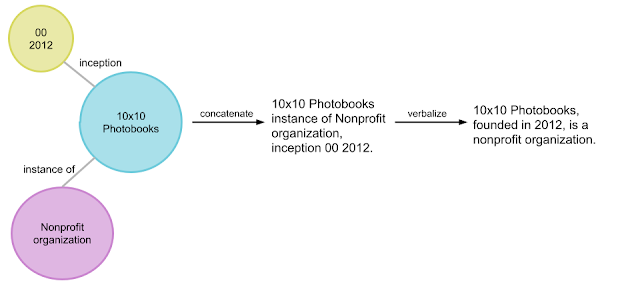
\includegraphics[width=0.65\linewidth,keepaspectratio]{llm47}
\end{center}	

{\tiny (Ref: KELM: Integrating Knowledge Graphs with Language Model Pre-training Corpora - Siamak Shakeri, Oshin Agarwal)}
\end{frame}

%%%%%%%%%%%%%%%%%%%%%%%%%%%%%%%%%%%%%%%%%%%%%%%%%%%%%%%%%%%
\begin{frame}[fragile]\frametitle{Use of KG in better usage of LLM, say, RAG}

Augmenting company information from KG and adding it into the prompt for better results.

\begin{center}
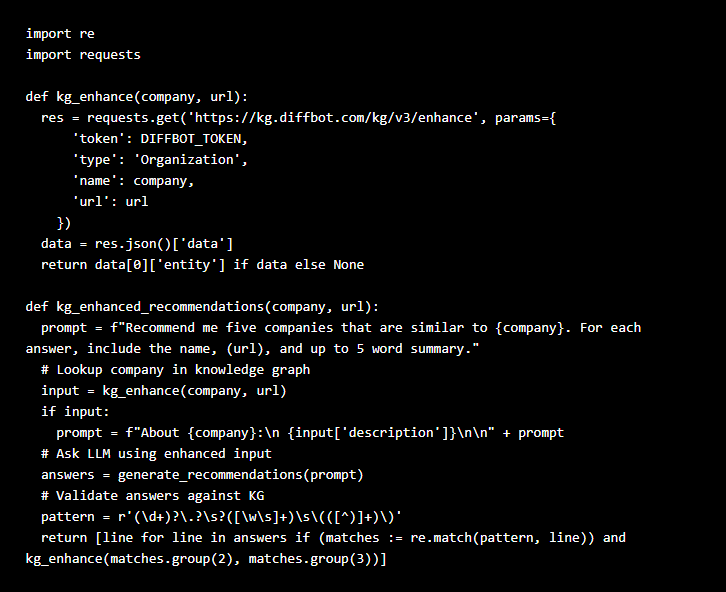
\includegraphics[width=0.65\linewidth,keepaspectratio]{llm51}
\end{center}	

{\tiny (Ref: Generating Company Recommendations using Large Language Models and Knowledge Graphs - Mike Tung)}

\end{frame}

%%%%%%%%%%%%%%%%%%%%%%%%%%%%%%%%%%%%%%%%%%%%%%%%%%%%%%%%%%%
\begin{frame}[fragile]\frametitle{Use of LLMs in building KG}

\begin{center}
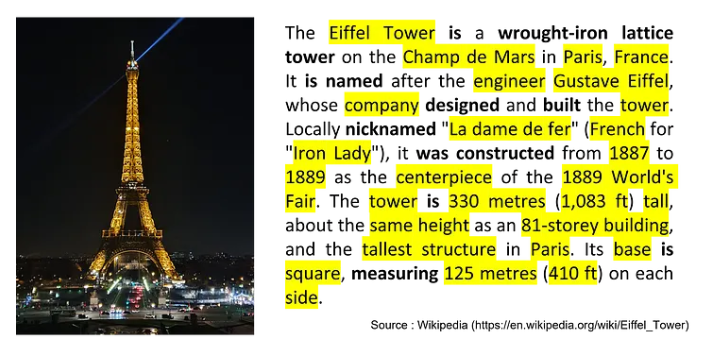
\includegraphics[width=\linewidth,keepaspectratio]{llm48}
\end{center}

{\tiny (Ref: Automatic Knowledge Graphs: The Impossible Grail - Patrick Meyer)}

\end{frame}

%%%%%%%%%%%%%%%%%%%%%%%%%%%%%%%%%%%%%%%%%%%%%%%%%%%%%%%%%%%
\begin{frame}[fragile]\frametitle{Unscrambling the Information}

Representing conceptual understanding, establishing connections between the LLM's numerical vectors and the KG's ontological classes.

\begin{itemize}
\item The Eiffel Tower is a wrought-iron lattice tower.
\item The Eiffel Tower is located on the Champ de Mars.
\item The Champ de Mars is located in Paris.
\item Paris is located in France.
\item The Eiffel Tower is named after the engineer Gustave Eiffel.
\item Gustave Eiffel’s company designed the Eiffel Tower.
\item Gustave Eiffel’s company built the Eiffel Tower.
\item The Eiffel Tower is locally nicknamed “La dame de fer”.
\item “La dame de fer” is the French for ”The Iron Lady”
\item The Eiffel Tower was constructed from 1887 to 1889.
\item The Eiffel Tower was constructed as centerpiece of 1889 World’s Fair.
\item The Eiffel Tower is 330 meters high.
\item The Eiffel Tower is the same height as an 81-storey building.
\item The Eiffel Tower is the tallest structure in Paris.
\item The base of the Eiffel Tower is a square.
\item The base of the Eiffel Tower measures 125 meters on each side.
\end{itemize}

{\tiny (Ref: Automatic Knowledge Graphs: The Impossible Grail - Patrick Meyer)}

\end{frame}

%%%%%%%%%%%%%%%%%%%%%%%%%%%%%%%%%%%%%%%%%%%%%%%%%%%%%%%%%%%
\begin{frame}[fragile]\frametitle{Populating KG}

\begin{center}
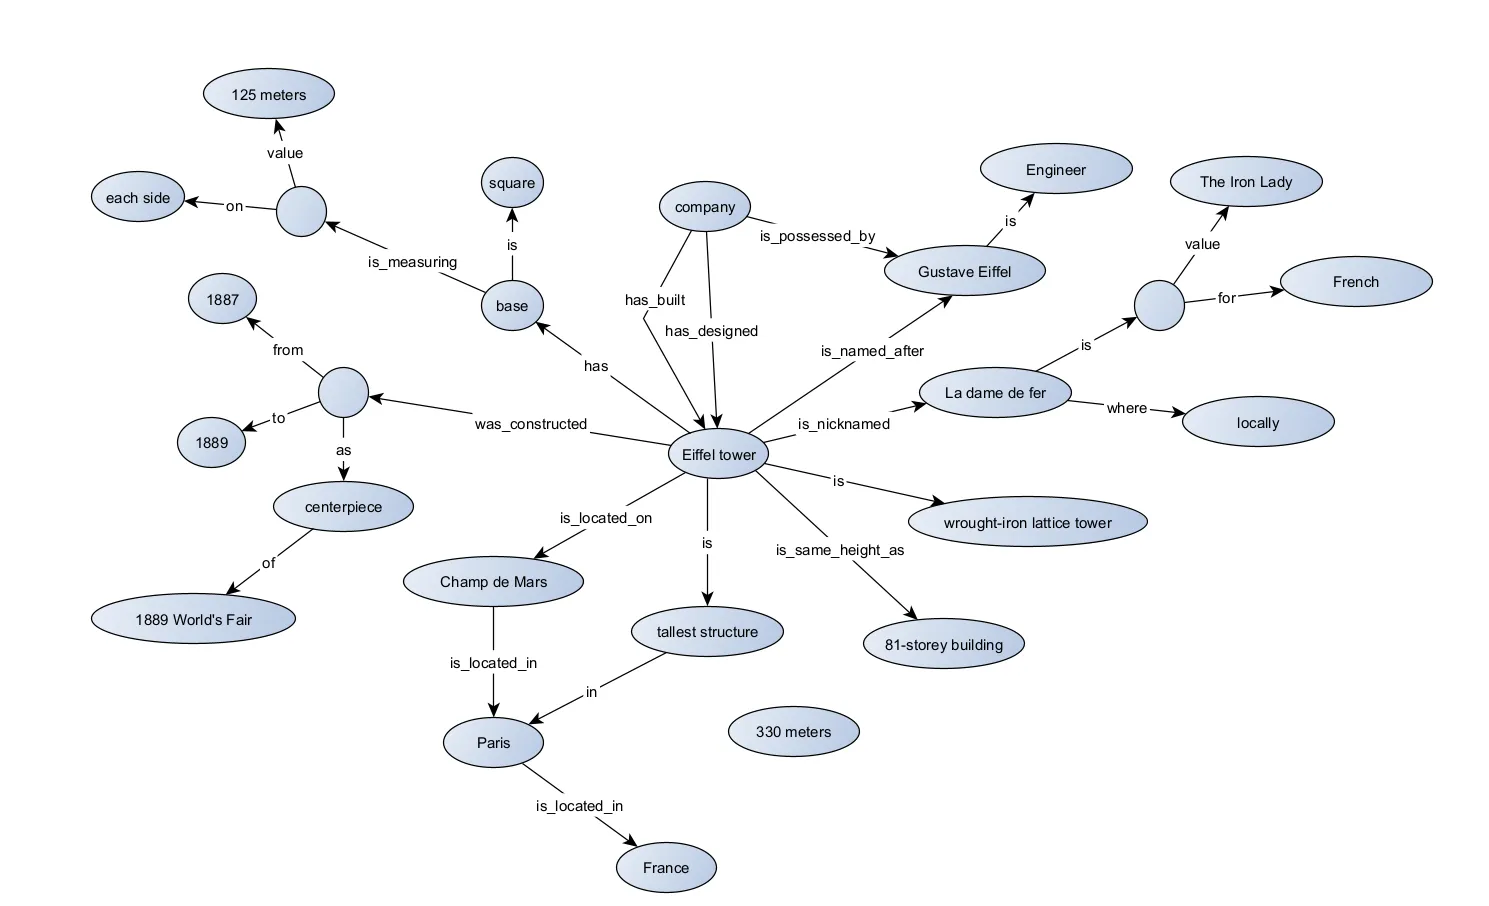
\includegraphics[width=\linewidth,keepaspectratio]{llm49}
\end{center}

{\tiny (Ref: Automatic Knowledge Graphs: The Impossible Grail - Patrick Meyer)}

\end{frame}

%%%%%%%%%%%%%%%%%%%%%%%%%%%%%%%%%%%%%%%%%%%%%%%%%%%%%%%%%%%
\begin{frame}[fragile]\frametitle{Populating KG is not easy}

\begin{center}
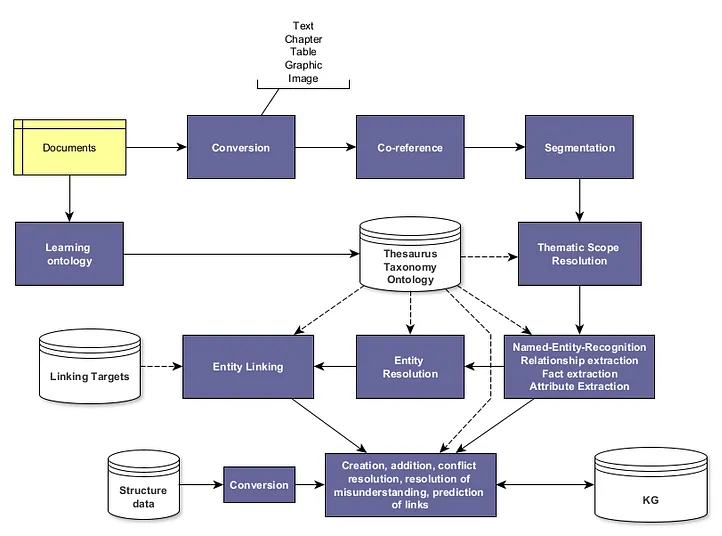
\includegraphics[width=0.8\linewidth,keepaspectratio]{llm50}
\end{center}

{\tiny (Ref: Automatic Knowledge Graphs: The Impossible Grail - Patrick Meyer)}

\end{frame}

%%%%%%%%%%%%%%%%%%%%%%%%%%%%%%%%%%%%%%%%%%%%%%%%%%%%%%%%%%%%%%%%%%%%%%%%%%%%%%%%%%
%%%%%%%%%%%%%%%%%%%%%%%%%%%%%%%%%%%%%%%%%%%%%%%%%%%%%%%%%%%
\begin{frame}[fragile]\frametitle{How?}

\begin{itemize}
\item Knowledge graph generation: Systematic approach for organizations.
\item Step 1: Ingest standard ontology (e.g., insurance risk).
\item Use LLM (e.g., GPT-3) to script and populate graph database.
\item Step 2: LLM acts as intermediate layer for natural language queries.
\item Customized creation and search queries on the graph.
\item Platform customization (e.g., Neo4j).
\end{itemize}
\end{frame}

%%%%%%%%%%%%%%%%%%%%%%%%%%%%%%%%%%%%%%%%%%%%%%%%%%%%%%%%%%%
\begin{frame}[fragile]\frametitle{Steps}

\begin{center}
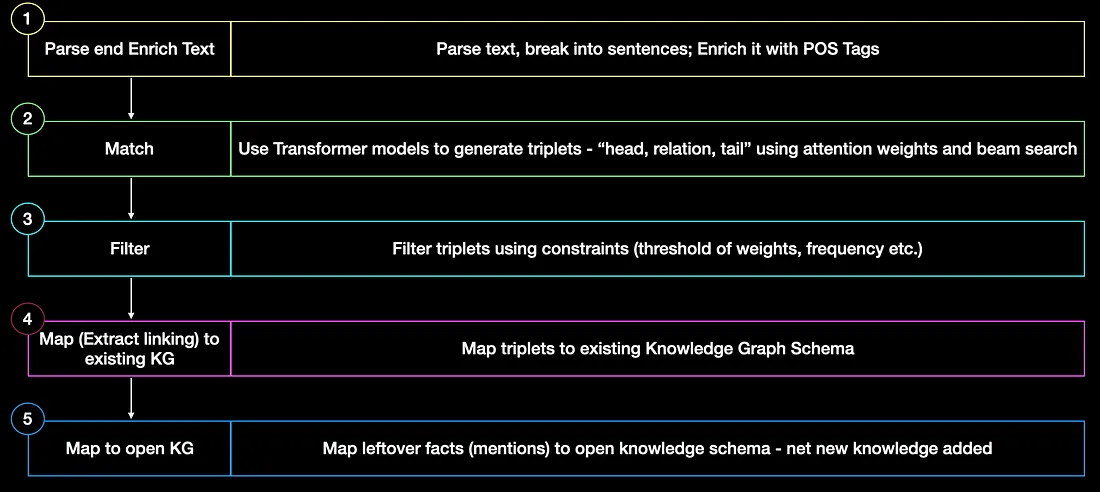
\includegraphics[width=\linewidth,keepaspectratio]{llm52}
\end{center}	

{\tiny (Ref: Language Models are Open Knowledge Graphs .. but are hard to mine! - Nikhil Dharap)}
\end{frame}



%%%%%%%%%%%%%%%%%%%%%%%%%%%%%%%%%%%%%%%%%%%%%%%%%%%%%%%%%%%%%%%%%%%%%%%%%%%%%%%%%%
%%%%%%%%%%%%%%%%%%%%%%%%%%%%%%%%%%%%%%%%%%%%%%%%%%%%%%%%%%%
\begin{frame}[fragile]\frametitle{Steps}

\begin{itemize}
\item Study ontology, identify entities and relations.
\item Build text prompt for LLM to generate schema and database.
\item Prompt includes ontology description, entities, relationships.
\item Clearly described in natural language for LLM understanding.
\item Include constraints (data types, unique/foreign keys).
\item Text prompt used as input for LLM to generate Cypher query.\end{itemize}
\end{frame}



%%%%%%%%%%%%%%%%%%%%%%%%%%%%%%%%%%%%%%%%%%%%%%%%%%%%%%%%%%%
\begin{frame}[fragile]\frametitle{Work-flow}

\begin{center}
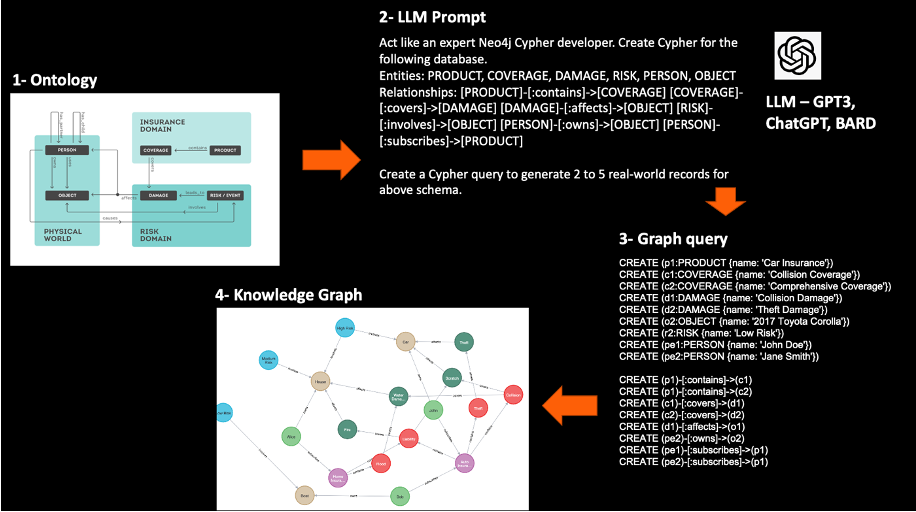
\includegraphics[width=\linewidth,keepaspectratio]{llm46}

{\tiny (Ref: How to use large language models and knowledge graphs to manage enterprise data - Dattaraj Rao, Persistent Systems)}
\end{center}
\end{frame}


%%%%%%%%%%%%%%%%%%%%%%%%%%%%%%%%%%%%%%%%%%%%%%%%%%%%%%%%%%%%%%%%%%%%%%%%%%%%%%%%%%
%%%%%%%%%%%%%%%%%%%%%%%%%%%%%%%%%%%%%%%%%%%%%%%%%%%%%%%%%%%
\begin{frame}[fragile]\frametitle{Pros and Cons}

\begin{itemize}
\item Standardization: Ensures consistent and standardized data.
\item Efficiency: Saves time and resources, ensures correct queries.
\item Intuitive querying: Reduces need for deep graph understanding.
\item Productivity: Updates knowledge graph with new data.
\item Modified Cypher query adds new nodes and edges.
\item Updated query ingested into graph database.
\end{itemize}
\end{frame}


%%%%%%%%%%%%%%%%%%%%%%%%%%%%%%%%%%%%%%%%%%%%%%%%%%%%%%%%%%%
\begin{frame}[fragile]\frametitle{Use of LLMs in better querying of KG}

\begin{itemize}
\item LLM converts verbose query to GraphQL syntax.
\item GraphQL performs information retrieval.
\item LLM converts GraphQL response to verbose answer.
\end{itemize}

	
{\tiny (Ref: Knowledge Graphs + Large Language Models = The ability for users to ask their own questions? - Peter Lawrence)}

\end{frame}

%%%%%%%%%%%%%%%%%%%%%%%%%%%%%%%%%%%%%%%%%%%%%%%%%%%%%%%%%%%
\begin{frame}[fragile]\frametitle{How?}

\begin{itemize}
\item Query : \lstinline|How is Valve-104 connected to Reflux-401?|
\item Using the OpenAI gpt-3.5-turbo LLM, provide the ontology of the RDF graph as the context prompt for the LLM.
\item Ask it to prepare some SPARQL
\end{itemize}	

\begin{lstlisting}
Sure! Here is an example of a SPARQL query that returns the sequence of nodes that connect two particular nodes, assuming that there is a unique path between them:
```
PREFIX connectivity: <http://example.org/ontology#>
SELECT ?path
WHERE {
  {
    <http://example.org/node1> (connectivity:connectedTo)+ ?path .
    ?path connectivity:connectedTo <http://example.org/node2> .
  }
}
```
\end{lstlisting}

\end{frame}

%%%%%%%%%%%%%%%%%%%%%%%%%%%%%%%%%%%%%%%%%%%%%%%%%%%%%%%%%%%
\begin{frame}[fragile]\frametitle{How?}

\begin{itemize}
\item Property path syntax: Find paths connecting two nodes.
\item \lstinline|(connectivity:connectedTo)+|: Traverses arbitrary length path with "connectedTo" property.
\item Query result: \lstinline|"?path"| variable represents sequence of connecting nodes (as URIs).
\item Assumes unique path between nodes.
\item Multiple paths or cycles may result in multiple/incorrect results.
\end{itemize}	

\end{frame}


% %%%%%%%%%%%%%%%%%%%%%%%%%%%%%%%%%%%%%%%%%%%%%%%%%%%%%%%%%%%%%%%%%%%%%%%%%%%%%%%%%%
% \begin{frame}[fragile]\frametitle{}
% \begin{center}
% {\Large Characteristics of KG + LLMs}

% {\tiny (Ref: LinkedIn posts by Tony Seale)}
% \end{center}
% \end{frame}

% %%%%%%%%%%%%%%%%%%%%%%%%%%%%%%%%%%%%%%%%%%%%%%%%%%%%%%%%%%%
% \begin{frame}[fragile]\frametitle{Training data for GPT}

% \begin{itemize}
% \item GPT learns from web pages, with 40\% containing JSON-LD islands.
% \item Reverse relationship: Use islands to connect GPT's embeddings to internal data.
% \end{itemize}
	  
% \end{frame}

% %%%%%%%%%%%%%%%%%%%%%%%%%%%%%%%%%%%%%%%%%%%%%%%%%%%%%%%%%%%
% \begin{frame}[fragile]\frametitle{Transformers as GNNs}

% \begin{itemize}
% \item Transformers: Analyze sentences by assigning word importance.
% \item Attention mechanism: Evaluates pairwise interactions between tokens.
% \item Interactions represented as edges in a complete graph.
% \item Transformers as graph-based models: Tokens as nodes, attention weights as edges.
% \end{itemize}
	  
% \end{frame}


% %%%%%%%%%%%%%%%%%%%%%%%%%%%%%%%%%%%%%%%%%%%%%%%%%%%%%%%%%%%
% \begin{frame}[fragile]\frametitle{Transparency and Explainability}

% \begin{itemize}
% \item Language models (e.g., ChatGPT) provide answers in interconnected node graphs.
% \item Visualizing connections reveals decision-making process.
% \item Helps address biases and ensure regulatory compliance.
% \end{itemize}
	  
% \end{frame}

% %%%%%%%%%%%%%%%%%%%%%%%%%%%%%%%%%%%%%%%%%%%%%%%%%%%%%%%%%%%
% \begin{frame}[fragile]\frametitle{Knowledge Management and Control}

% \begin{itemize}
% \item Language models (e.g., ChatGPT) provide answers in interconnected node graphs.
% \item Visualizing connections reveals decision-making process.
% \item Helps address biases and ensure regulatory compliance.
% \end{itemize}
	  
% \end{frame}

% %%%%%%%%%%%%%%%%%%%%%%%%%%%%%%%%%%%%%%%%%%%%%%%%%%%%%%%%%%%
% \begin{frame}[fragile]\frametitle{Alignment with Ontological Worldview}

% \begin{itemize}
% \item Leverage Knowledge Graph ontology to constrain the language model.
% \item Alignment maintains logical consistency with organization's perspective.
% \item Prevents retrieval of outdated or incorrect information.
% \end{itemize}
	  
% \end{frame}

% %%%%%%%%%%%%%%%%%%%%%%%%%%%%%%%%%%%%%%%%%%%%%%%%%%%%%%%%%%%
% \begin{frame}[fragile]\frametitle{Alignment with Ontological Worldview}
% \begin{itemize}
% \item Knowledge Graph ontology constrains language model.
% \item Alignment ensures logical consistency with organization's perspective.
% \item Prevents retrieval of outdated or incorrect information.
% \end{itemize}
% \end{frame}

% %%%%%%%%%%%%%%%%%%%%%%%%%%%%%%%%%%%%%%%%%%%%%%%%%%%%%%%%%%%
% \begin{frame}[fragile]\frametitle{Risk Assessment and Compliance}
% \begin{itemize}
% \item Knowledge graphs enable comprehensive risk assessment.
% \item Empower proactive identification of sensitive information, compliance risks, and ethical challenges.
% \item Mitigate potential issues before escalation.
% \end{itemize}
% \end{frame}

% %%%%%%%%%%%%%%%%%%%%%%%%%%%%%%%%%%%%%%%%%%%%%%%%%%%%%%%%%%%
% \begin{frame}[fragile]\frametitle{Ethical and Fair AI}
% \begin{itemize}
% \item Knowledge graphs encode ethical guidelines and fairness constraints into Ontology that upholds organization's standards.
% \item Language model adheres to ethical principles and promotes fairness.
% \end{itemize}
% \end{frame}

% %%%%%%%%%%%%%%%%%%%%%%%%%%%%%%%%%%%%%%%%%%%%%%%%%%%%%%%%%%%
% \begin{frame}[fragile]\frametitle{Challenges}
% \begin{itemize}
% \item Balancing innovation and risk management in rapidly evolving landscape
% \item Language models like ChatGPT offer productivity and customer experience benefits
% \item Robust governance frameworks are essential to mitigate risks
% \end{itemize}
% \end{frame}

% %%%%%%%%%%%%%%%%%%%%%%%%%%%%%%%%%%%%%%%%%%%%%%%%%%%%%%%%%%%
% \begin{frame}[fragile]\frametitle{Knowledge Graphs: A Safe Path Forward}
% \begin{itemize}
% \item Knowledge graphs: Safe and effective approach for harnessing language models
% \item Leverage capabilities for navigating risk and governance
% \item Unlock benefits of AI-driven language models
% \end{itemize}
% \end{frame}

% %%%%%%%%%%%%%%%%%%%%%%%%%%%%%%%%%%%%%%%%%%%%%%%%%%%%%%%%%%%
% \begin{frame}[fragile]\frametitle{Generalized or Specific}
% \begin{itemize}
% \item Large Language Models (LLMs): Generalization, flexibility, and creativity, but suffer from hallucinations, unreliability, and staleness.
% \item Databases: Accuracy, speed, and reliability, but lack adaptability and intelligence.
% \item Bridge the gap with graphs: Integrate LLMs with internal data through Knowledge Graphs.
% \item Working Memory Graph (WMG): Combines strengths of LLMs and databases for tasks.
% \item WMG construction: LLM processes question, returns node graph with URLs as identifiers.
% \item Ground truths: Stored in the organization's Knowledge Graph, linked to URLs.
% \item Conceptual understanding: WMG incorporates nodes connecting LLM's vectors and KG's classes.
% \end{itemize}
% \end{frame}


%%%%%%%%%%%%%%%%%%%%%%%%%%%%%%%%%%%%%%%%%%%%%%%%%%%%%%%%%%%
\begin{frame}[fragile]\frametitle{KG + LLM @ Neo4j}
\begin{itemize}
\item https://github.com/neo4j/NaLLM
\item Explore, develop, and showcase practical uses of LLMs with Neo4j data science algorithms.
\item Strategy can yield substantial breakthroughs for businesses.
\item Enhance accuracy, transparency, and predictability of model output.
\item Open up new use-cases for LLMs and databases.
\item Real-world use-cases:

	\begin{itemize}
	\item Natural Language Interface: "Talk to your database" with generated queries based on user questions and inferred database schema.
	\item Creating Knowledge Graph from Unstructured Data: LLMs decipher entities, discern relationships, and eliminate redundancies by recognizing duplicates.
	\end{itemize}

\end{itemize}
\end{frame}

%%%%%%%%%%%%%%%%%%%%%%%%%%%%%%%%%%%%%%%%%%%%%%%%%%%%%%%%%%%
\begin{frame}[fragile]\frametitle{Example}

Wisecube's Unified Approach for Leveraging Large Language Models to Augment its Biomedical Knowledge Graph

\begin{center}
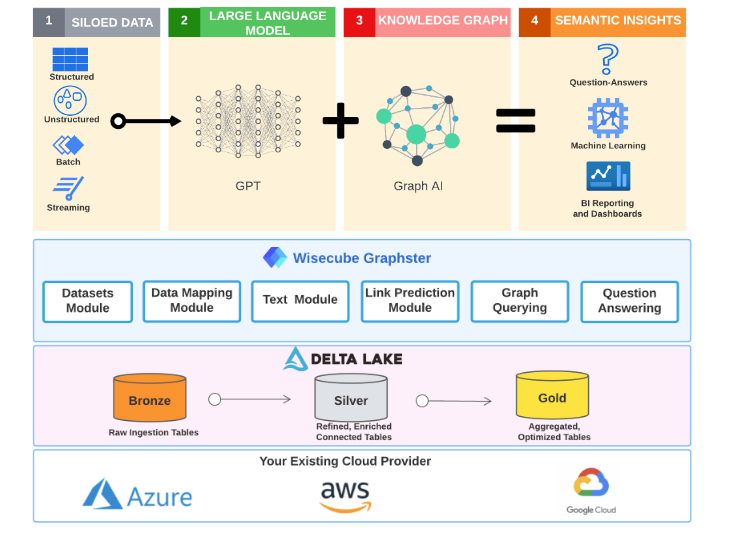
\includegraphics[width=0.7\linewidth,keepaspectratio]{llm102}
\end{center}	

{\tiny (Ref: Combining Large Language Models and Knowledge Graphs - Haziqa Sajid )}

\end{frame}
